%
% anwendungen.tex -- Paper zum Thema Optische Fourier-Transformation <opt>
%
% (c) 2023 Marco Niederberger, Yanick Schoch; OST Ostschweizer Fachhochschule
%
% !TEX root = ../../buch.tex
% !TEX encoding = UTF-8
%
\section{Anwendungen}
\label{opt:section:anwendungen}
\rhead{Praktische Anwendungen}

Nach den Grundlagen und den durchgeführten Versuchen wird in diesem Abschnitt auf die tatsächlichen Anwendungsgebiete eingegangen.
Es werden drei verschiedene Bereiche erläutert, in denen die Beugung und die optische Fourier-Transformation zur Anwendung kommen.
Das Spektrum reicht dabei von der Mustererkennung über neuronale Netze bis hin zu Artefakten auf Weltraumbildern.

\subsection{Mustererkennung}
Die schnelle Erstellung einer Fourier-Transformation kann für die Erkennung von vordefinierten Mustern verwendet werden.
Dabei wird das zu untersuchende Muster auf die Bildebene der ersten Linse gelegt. 
In Abbildung \ref{opt:fig:4fAufbau} als \emph{Originalbild} bezeichnet.
In der Fourier-Ebene ist anschliessend die bekannte Fourier-Transformation ersichtlich.
Abbildung \ref{opt:fig:patternYT} zeigt drei verschiedene solche Transformationen.
Mittels einer Maskierung der jeweiligen Transformationen und einer anschliessenden Helligkeitsmessung kann auf das gesuchte Muster geschlossen werden.
In \cite{opt:YT:PatternRecognition} wird dies anhand eines Versuches mit den Buchstaben A und B visualisiert.
Die Geschwindigkeit hierbei ist nicht mehr durch eine elektronische Schaltung gegeben.
Einzig limitierend ist die Geschwindigkeit, mit der das Licht durch den Versuchsaufbau gelangt, plus die Anstiegszeit der Photodiode.
Abgeschätzt mit einer Distanz von 20 cm und einer Anstiegszeit von 100 ps liegt die totale Zeit pro Erkennung bei rund 900 ps.
Dies entspricht einer Frequenz im Bereich von 1 GHz, mit welcher Muster erkennt werden können.

\begin{figure}
    \centering
    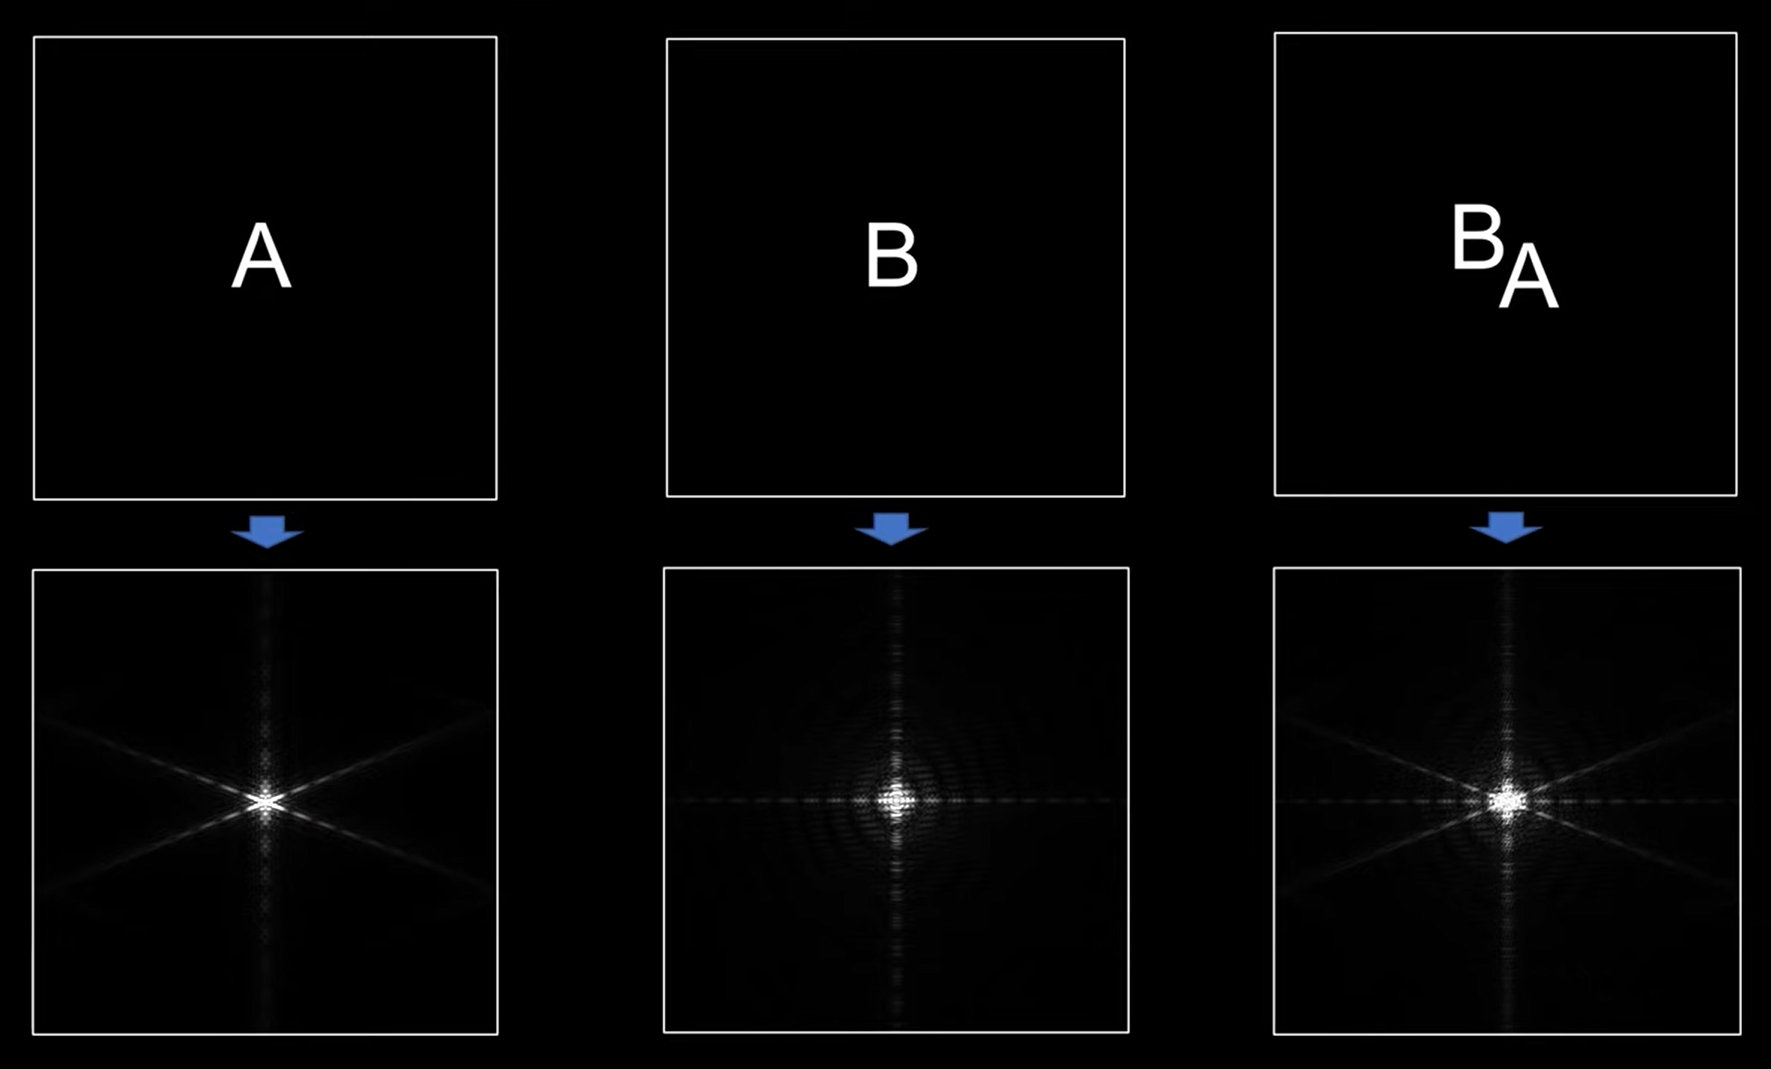
\includegraphics[width=0.6\textwidth]{papers/opt/images/pattern_YT.png}
    \caption{Frequenzspektrum der verschiedenen Muster. 
    Mittels einer Maskierung und einer Helligkeitsmessung kann das entsprechende Muster detektiert werden.}
    \label{opt:fig:patternYT}
\end{figure}

\subsection{Diffractive deep neural network}
Beim obenstehenden Beispiel wurde nur mit einer einzelnen Blende gearbeitet, um das gesuchte Muster zu erkennen.
In \cite{opt:Lin.2018} wurde dieser Ansatz durch Lin et al. erweitert und mit mehreren Ebenen erfolgreich getestet.
Abbildung \ref{opt:fig:handwriting}a zeigt den schematischen Aufbau mit fünf Ebenen.
Der Grundsatz bleibt gleich; kohärentes Licht wird von einer ersten Input Ebene gebeugt und anschliessend an fünf weiteren Ebenen.
Dies entspricht im Ansatz den verschiedenen verknüpften Neutronen eines neuronalen Netzwerkes.
Nach den Beugungsebenen wird das Licht durch mehrere Detektoren erkannt.
Lin et al. konnten damit erfolgreich handschriftliche Zahlen detektieren.
Mittels fünf aufeinanderfolgenden Ebenen und zehn Detektoren gelang es ihnen, mehr als 90\% der Schriften korrekt zuzuordnen.
Dieser Wert ist relativ schlecht im Vergleich zu konventionellen Methoden der Mustererkennung.
Angesichts der erreichten Erkennungsgeschwindigkeit ist dies jedoch trotzdem sehr beachtlich.

\begin{figure}
    \centering
    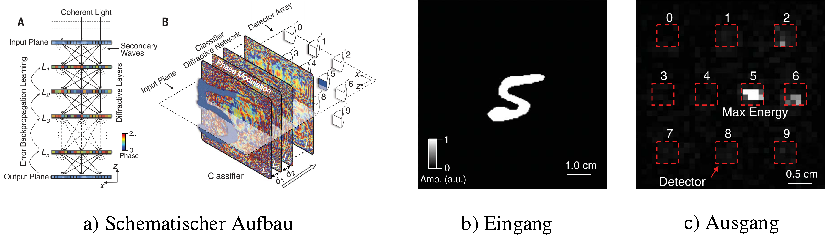
\includegraphics[width=\textwidth]{papers/opt/images/handwriting.pdf}
    \caption{Abbildung a) zeigt den Aufbau, wie er in \cite{opt:Lin.2018} verwendet wurde, um handschriftliche Ziffern zu erkennen.
    Abbildung b) und c) zeigen den Eingang sowie das Bild auf dem Detektor des Systems}
    \label{opt:fig:handwriting}
\end{figure}

\subsection{James-Webb-Weltraumteleskop}
Eine weiteres Beispiel der Beugung befindet sich aktuell im Weltraum.
Auf den Bildern des James-Webb-Weltraumteleskops (JWST) sind jeweils sechs (beziehungsweise drei durchgehende) helle Strahlen ersichtlich.
Diese werden durch die Geometrie des Spiegels erzeugt.

Das Teleskop besteht aus einem sechseckigen Hauptspiegel mit einem Loch sowie einem vorgelagerten Spiegel.
Dieser wiederum ist mit drei Stützen mit der Struktur des JWST verbunden.
Dabei wurden zwei Stützen so platziert, dass deren Strahlen deckungsgleich mit denjenigen des Hauptspiegels sind.
Die dritte Stütze ist senkrecht montiert und somit nicht mit einem Strahl des Hauptspiegels deckungsgleich.
Dies ist auf den Bildern als vierter Strahl zu sehen.
Durch die Überlagerung dieser beiden Effekte ergeben sich in Abbildung \ref{opt:fig:jwst} die charakteristischen Strahlen, welche auf
den veröffentlichten Bildern des JWST zu sehen sind.

Im Gegensatz dazu sind beim Hubble Teleskop vier (beziehungsweise zwei durchgehende) Strahlen ersichtlich.
Dies kommt davon, dass bei diesem Teleskop der Sekundärspiegel mittels vier Stützen mit der restlichen Struktur verbunden ist.

\begin{figure}
    \centering

    \subfigure{
        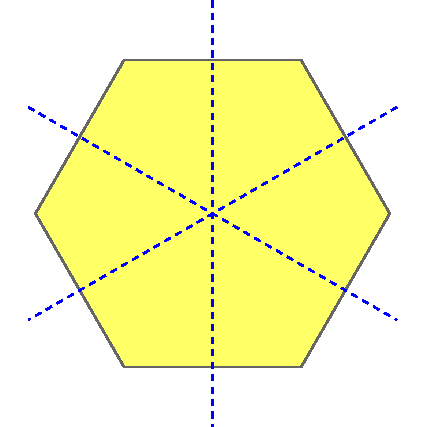
\includegraphics[page=1, width=0.3\linewidth]{papers/opt/images/jwst_sechseck.pdf}
    }
    \hfill
    \subfigure{
        \includegraphics[page=2, width=0.3\linewidth]{papers/opt/images/jwst_sechseck.pdf}
    }
    \hfill
    \subfigure{
        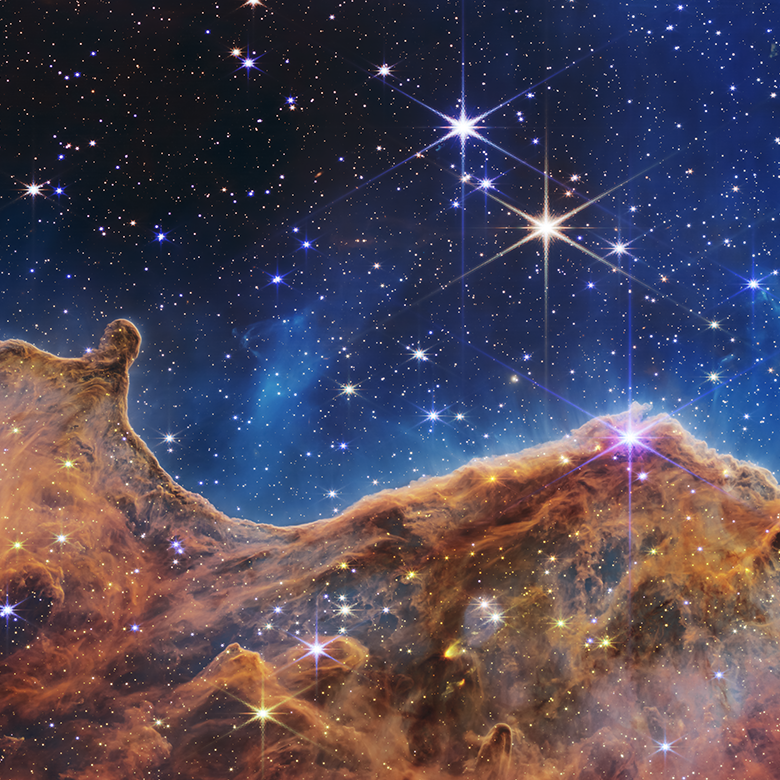
\includegraphics[width=0.3\linewidth]{papers/opt/images/jamesWebb_cropped_publicDomain.png}
    }
    \caption{Links die Strahlen der sechs Aussenkanten, mittig der drei Stützen sowie rechts eine Aufnahme der NASA (Public Domain)
        des James-Webb-Weltraumteleskop mit den charakteristischen Strahlen.}
    \label{opt:fig:jwst}
\end{figure}
